\chapter{Results}
\label{chap:phages_results}

This chapter first presents the outcomes of our model in a well-mixed chemostat environment, before focusing on the traveling wave dynamics and observing a protective effect of resistant bacteria. This effect is further investigated and we were able to show that the origin is a decoupling of phage and bacterial front, resulting in a widening of the sensitive peak in the system. Furthermore, we were able to show that resistant bacteria are necessary to observe this effect, while nutrient reduction only reproduces a weak effect. However, our findings are limited by the ability of phages to infect and replicate in non-growing bacteria.

\section{Chemostat observations}
First we study the system in a well-mixed, chemostat environment. As expected, when increasing the dilution rate in a chemostat with only sensitive bacteria, we observe a monotonic decline in the amount of sensitive bacteria in a steady state in the chemostat~(Figure~\ref{fig:results_chemostat_traveling_wave}a, black curve). When adding phages, we observe an overall decline in sensitive bacteria. When the dilution rate is low, there are significantly less sensitive bacteria. However, in contrast to the sensitive only scenario, the amount of sensitive bacteria increases with increasing dilution rate up to a point where it is identical to this scenario. Then it declines in the same pattern with increasing dilution rate~(Figure~\ref{fig:results_chemostat_traveling_wave}a, red curve). This indicates a lower wash out rate for phages than for sensitive bacteria. Lastly, when adding resistant bacteria with equal fitness to the system, we observe a similar pattern but the amount of sensitive bacteria is lower at any point, indicating the competition over nutrients with resistant bacteria~(Figure~\ref{fig:results_chemostat_traveling_wave}a, blue curve). The peak of sensitive bacteria is reached at a lower dilution rate than without resistant bacteria. Choosing now the dilution rate at this peak, we study the change of sensitive bacteria when changing the fitness of the resistant bacteria in the system. We observe sensitive bacteria in the system for resistant fitness values lower than equal fitness and then a sharp decline at equal fitness~(Figure~\ref{fig:results_chemostat_traveling_wave}b, blue curve). This shows that resistant bacteria outcompete sensitive bacteria in a well-mixed environment as described in previous works.
\begin{figure}
\centering
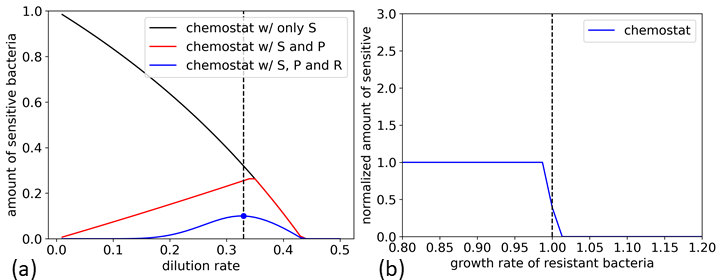
\includegraphics[width=\linewidth]{graphics/2025_09_29_phages_fig2.png}
\caption{\textbf{Chemostat shows resistant bacteria outcompete sensitive} (a) shows the amount of sensitive bacteria depending on the dilution rate for different scenarios. In black is a scenario with only sensitive bacteria, in red a scenario with phages and sensitive bacteria and in blue a scenario with phages, sensitive and resistant bacteria. (b) shows the normalized amount of sensitive bacteria changing with the growth rate of resistant bacteria for a chemostat (blue). The chemostat shows a decrease at the point of equal fitness of resistant and sensitive bacteria. This indicates that sensitive bacteria go extinct ones resistant bacteria are fit enough to take over.}
\label{fig:results_chemostat_traveling_wave}
\end{figure}

\section{Traveling wave dynamics}
Simulating the model with diffusion and initial conditions such that the nutrients are constant and bacteria and phages are concentrated on one side of the system, we obtain a traveling wave dynamics, where bacteria and phages travel together through the system, invading previously unoccupied regions. The nutrients are receding, allowing a sensitive front to be formed. Trailing behind is a phage front which restricts the sensitive bacteria to a narrow region between its front and the phage front. In a narrow intermediate region, a small peak of infected bacteria forms. Resistant bacteria travel uninhibited by phages through the system. These dynamics resemble previously observed experimental results.

\begin{figure}
\centering
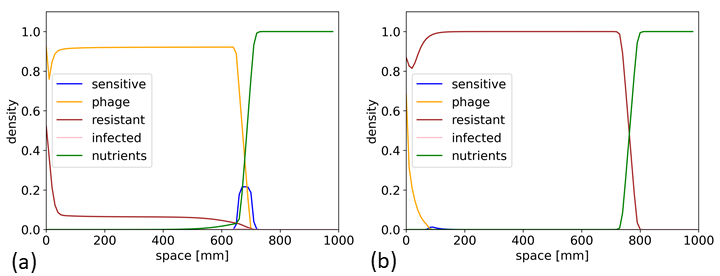
\includegraphics[width=\linewidth]{graphics/2025_09_29_phages_fig3.png}
\caption{\textbf{Traveling wave dynamics for $\lambda_r \approx 0.617$ and $\lambda_r \approx 1.13$} This figure shows two snapshots of the dynamics formed when solving the model for different $\lambda_r$. (a) shows a scenario with low $\lambda_r$, revealing the survival of a traveling sensitive wave which propagates ahead of a phage wave and a wave of resistant bacteria. Where phages caught up, infected bacteria are formed but they do not reach the sensitive front. (b) shows a scenario with high $\lambda_r$, revealing the overtake of the system by resistant bacteria and phages and sensitive bacteria not able to propagate due to nutrient limitations and slowly going extinct.}
\label{fig:traveling_wave_dynamics}
\end{figure}

\section{Protection by resistant bacteria}
\label{sec:protective_effect}
Using the established model, we can vary the growth rate of resistant bacteria relative to sensitive bacteria. For low growth rates, we observe survival of sensitive bacteria. For resistant bacteria growth rates higher than the sensitive bacteria growth rate, we see no survival of sensitive bacteria in the system. Surprisingly, for growth rates just below the expected transition point at equal growth rate, we observe a protective effect of the resistant bacteria resulting in an increased amount of sensitive bacteria (Figure~\ref{fig:results_chemostat_traveling_wave}b, red curve). When studying the change of the amount of sensitive bacteria around the maximum over time (Figure~\ref{fig:results_peak_change_height_width}a), we observe a change from a regime where the amount stabilizes quickly and stays constant over a regime where the amount of bacteria constantly linearly increases over time to a regime where after an initial increase, the amount collapses and plateaus or goes towards extinction (Figure~\ref{fig:results_peak_change_height_width}b).

\begin{figure}
\centering
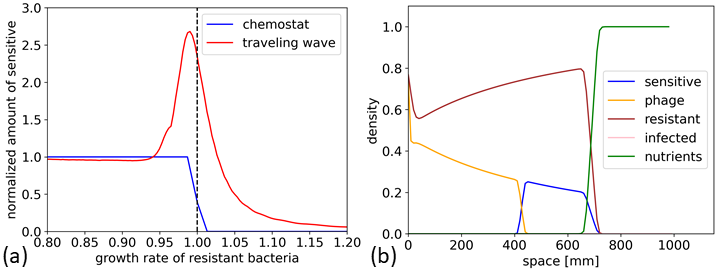
\includegraphics[width=\linewidth]{graphics/2025_09_29_phages_fig4.png}
\caption{\textbf{Resistant bacteria protect sensitive bacteria in a structured environment} (a) shows the comparison between a chemostat and the traveling wave scenario in a spatially structured environment. The traveling wave scenario reveals a protective effect resulting in an almost three-fold increase in sensitive bacteria just before the point of equal fitness. When resistant bacteria grow faster, sensitive bacteria go extinct. (b) shows the dynamics for $\lambda_r \approx 0.99$, at the peak of protection, revealing a long-term transition state which results in a wider region of sensitive bacterial presence.}
\label{fig:protective_effect}
\end{figure}

\section{Widening causes protection}
When studying the width and height of the traveling wave of bacteria, we observe the explanation for the observed protective effect. Monitoring the observed protective peak, we see a transition from a narrow, high peak to a shallow but wide peak of sensitive bacteria with increasing resistant growth rate. Once resistant bacteria grow faster, the sensitive peak disappears. The linear increase in width suggests that the two wave fronts, sensitive bacteria and phages, separated and travel with constant but different speeds. Indeed, measuring the speeds of these two fronts, we observe that the phage front slows down at a lower resistant growth rate than the sensitive bacteria front. However, measuring the difference in speed, we observe that the maximal difference is at a higher growth rate than the observed protective effect. However, as is apparent from our previous height and width analysis, for higher growth rates, the peak is diminished and indeed, multiplying speed with height as a new quantification of the effect, we observe an effect for those growth rates which also reveal the protective effect. So overall, the product of speed difference and height explains the observed protective effect. 

\begin{figure}
\centering
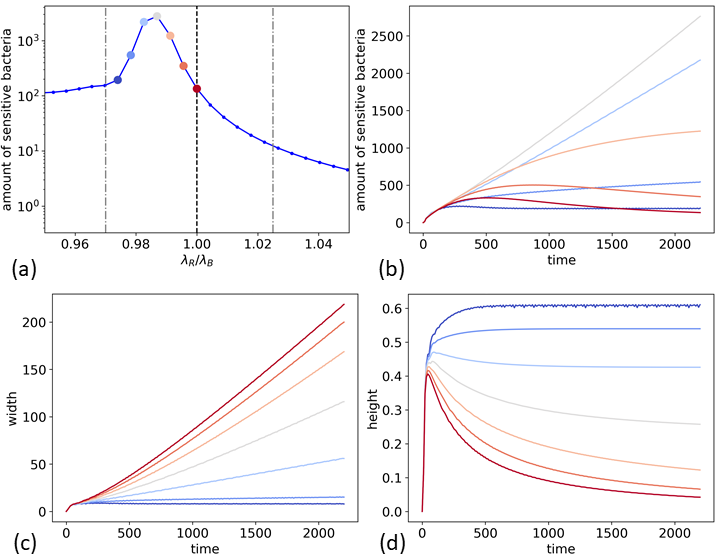
\includegraphics[width=\linewidth]{graphics/2025_09_29_phages_fig5.png}
\caption{\textbf{Closer examination of the protective peak reveals widening} (a) shows a focused view on the protective peak, described earlier. (b) shows the amount of sensitive bacteria over time for the points indicated with different colors in (a). (c) and (d) show the width and height respectively over time for these chosen points.}
\label{fig:results_peak_change_height_width}
\end{figure}

\begin{figure}
\centering
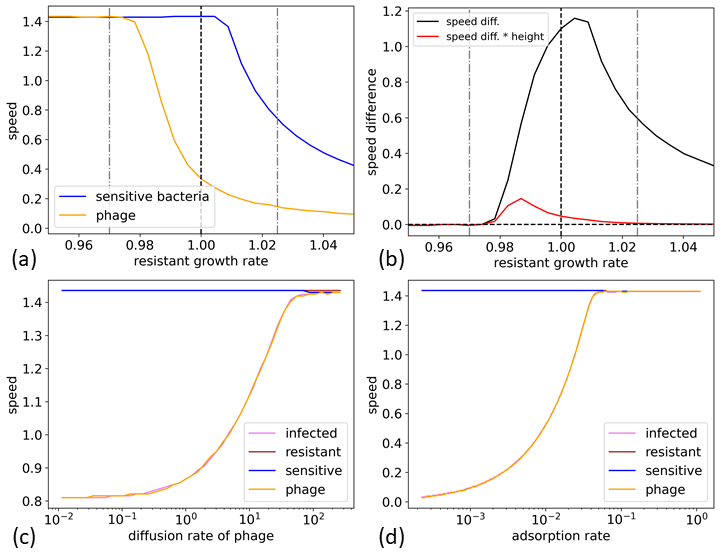
\includegraphics[width=\linewidth]{graphics/2025_09_26_phages_fig4.png}
\caption{\textbf{Speed difference identified as cause for widening} (a) shows the speed of the expanding wave front of phages and of sensitive bacteria as a function of resistant growth rate, (b) shows the difference between these two speeds and the new measurement of the product between speed difference and height, (c) and (d) show the speed for changing two important parameters, phage diffusion and infection rate respectively.}
\label{fig:results_speed_height}
\end{figure}

\section{Nutrient sparsity weakly protects}
Previous models, studying a phage wave invading an exponentially growing, sensitive population~\cite{Claydon2021-cu} show a separation between the speed of the receding sensitive wave and the speed of the advancing phage wave without resistant bacteria present in the system. Motivated by this results, we are studying in this section, whether we can observe the protective effect in a system without resistant bacteria when instead limiting the available nutrients. Lowering the initially available nutrients in the system, reduces the speed of both waves while for very nutrient concentrations and therefore low speeds a minor speed difference occurs. However, this effect is much smaller than the effect obtained when resistant bacteria are present in the system. Therefore, we conclude that resistant bacteria are necessary to observe the protective effect.
\section{Impact of resistant diffusion rate}
Wave speed and therefore also the bacterial competition are known to not only depend on the growth rate but also on the diffusion rate of the bacteria. Therefore, we analysed the impact changes in both of these parameters on the amount of sensitive bacteria and we found a clear phase transition from a parameter regime in which sensitive bacteria survive to a parameter regime in which sensitive bacteria do not survive~(Figure~\ref{fig:results_heatmap_effect}). Close to the transition interface, we observe the protective effect we previously described in section~\ref{sec:protective_effect}. There seems to be a linear correlation between growth rate and diffusion rate for low growth rates, in agreement with the theoretical results for the KPP-equation. However, for higher growth rates, this linear relation collapses and we observe a dominant effect of growth rate rather than diffusion rate.
\begin{figure}
\centering
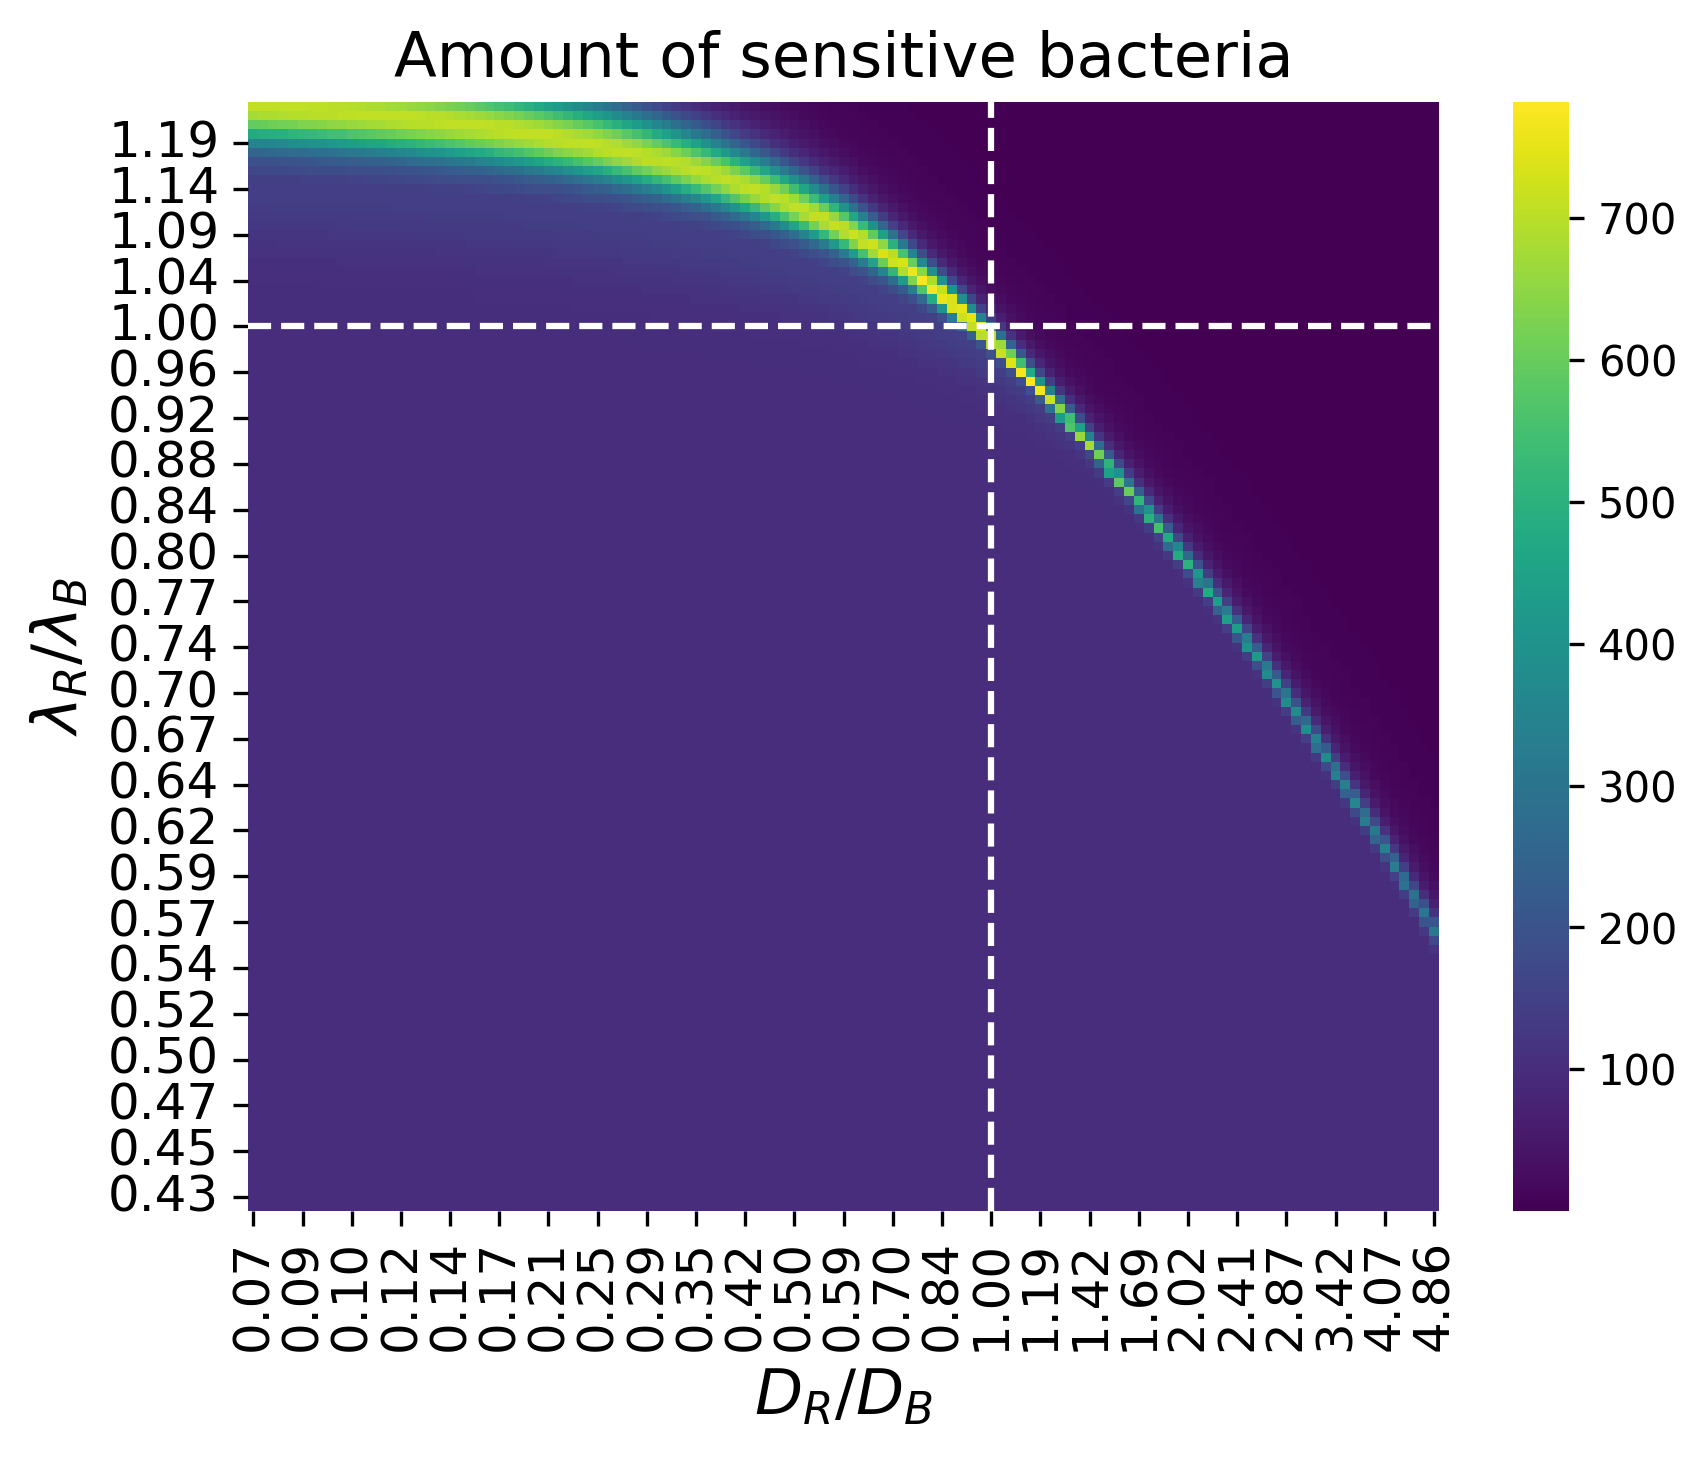
\includegraphics[width=\linewidth]{graphics/2025_09_26_phages_fig5.png}
\caption{\textbf{Phase transition with two parameters with protective effect} The heatmap shows the amount of sensitive bacteria for different combinations of resistant growth rate and resistant diffusion rate, indicating a phase transition from a region with sensitive bacteria to a region without. At the interface, we observe an increase in sensitive bacteria.}
\label{fig:results_heatmap_effect}
\end{figure}

\section{Impact of parameters}
Our model includes several other parameters, some of which could impact the dynamics. In this section, we are focusing on the phage diffusion rate and the infection rate, both known as parameters whose change can change the phage speed and indeed, we observe that the described protective effect vanishes when phages diffuse faster~(Figure~\ref{fig:results_speed_height}c) or the infection rate is higher~(Figure~\ref{fig:results_speed_height}d). However, while we observe a similar impact of the infection rate in a scenario without resistant bacteria, we do not observe this impact for the phage diffusion rate. 
\section{Limitations}
Some phages replicate only on growing bacteria due to the dependence on the replication machinery of bacteria. Therefore, we explored such a scenario by limiting the infection rate indirectly through a dependence on the nutrients with:
\begin{equation}
    \eta = \eta_0 \frac{n}{K_n + n}
\end{equation}
where $\eta_0$ is set to be the same infection rate as in the scenario without this dependence.
In this scenario, we were unable to observe the protective effect and we rather see a phase transition due to fitness of resistant and sensitive bacteria. Furthermore, if comparing it to a no-phage scenario, where bacteria compete without phages in the system, we see only minor differences between these cases.
This means that the ability for phages to replicate on non-growing bacteria is crucial for the protective effect to exist.

% \chapter{A main chapter}
% \label{chap:firstchap}

% \section{Introduction}

% You might have a per-chapter mini-intro, possibly tying in to the relevant part of the general intro.

% \section{A section}

% \lipsum[1]

% Let's cite a source: \cite{Yao1977}. And now,  let's introduce a (numbered) equation. It will use \gls{symb:c}, which is one of the entries in the ``\nameref{chap:notation-and-abbreviations}'' list. The equation will be in ``display math'' mode, using the \texttt{align} environment.

% \begin{align}
% \label{eq:emc2}
% e &= mc^2
% \end{align}
% \begin{notes}
% \item	Are you seeing a problem with the equation numbering? In some TeX processors and on some platforms, there may be a layout error, so that instead of ``(3.1)'' you get ``)3.1)'' or some other flipping of directions. Specifically, \url{http://overleaf.com} suffers from this problem (at least until 2020). Please make sure and use an appropriate TeX distribution that's up-to-date. Specifically, recent TeXLive versions work fine. On Overleaf, you can switch TeXLive versions using the main menu.
% \end{notes}

% Alternatively, we can use the \texttt{equation} environment with a label. For this to work, our theorem layout package, \texttt{ntheorem}, must be used with the \texttt{amsmath} option. Having done so, let's try our equation:
% \begin{equation}
% \label{eq:power-series}
% f(x)=\sum_{i=0}^{\infty} a_i x^i
% \end{equation}
% Equation \ref{eq:power-series} is a typical power series.

% In \autoref{sec:thm-like} below, we will state some theorems.

% \section{Results... and theorem-like environments}
% \label{sec:thm-like}

% What's so special about the theorem-like environments used here? There are several packages which offer the capability of defining these, mainly \texttt{amsthm}, \texttt{ntheorem} and also \texttt{thmtools}. (The last is probably also the most feature-full and versatile, but I'm not familiar with it and the first two are the popular ones.) Many people writing a Technion thesis start with \texttt{amsthm}, only to find out it has conflicts with Hebrew... also, there's the issue of aliasing (same counter for lemmata and theorems, but having \texttt{{\textbackslash}autoref} and similar commands know what they're referencing.) This is all neatly resolved in \texttt{iitthesis-extra.sty} with \texttt{amsthm}-like-looking environments actually done with nthrerom.

% \begin{theorem}
% \label{thm:first}
% This is the first numbered theorem in this thesis.
% \end{theorem}

% And we can refer to it using \texttt{ref}: \ref{thm:first} and get the number, or use hypertex's \texttt{autoref}: \autoref{thm:first}.

% \begin{corollary}
% \label{cor:first}
% There are no lemmata appearing before theorems in this thesis.
% \end{corollary}

% \begin{theorem*}
% This is the second theorem, unnumbered.
% \end{theorem*}

% \begin{theorem*}[\protect{\cite[Theorem 2]{Knuth1973}}]
% This is an unnumbered theorem cited from elsewhere. \qbfox{1} ... and it was Knuth's dog.
% \end{theorem*}

% \begin{note}
% This is a note environment.  \qbfox{2}
% \end{note}

% \begin{definition}
% \label{def:first}
% An \emph{quick brown fox} is a fox which is not only fast and agile but is also characterized by brown fur. Such foxes sometimes tend to jump over lazy dogs.
% \end{definition}

% \begin{lemma}
% \label{lem:first}
% This is a lemma. \qbfox{2}
% \end{lemma}

% Even though \autoref{lem:first} and \autoref{def:first} share the ``same'' counter, when referring to them, their names are used automagically.

% Here's a proof of the lemma:
% \begin{proof}%[lem:natural:blowups-preserve-distance-on-average]
% \lipsum[2]
% 	It's common to conclude proofs with a QED symbol --- typically a full or an empty black square. To do so, append the command \verb|\qed| after the last sentence of your proof; or, alternatively, you can use some \LaTeX{} trickery in the definition of the proof environment to ensure this symbol is appended to all proofs. This is done in the \texttt{misc/iitthesis-extra.sty} style file, which is used by this template. You will see the result as a black square at the end of this proof environment.
% \end{proof}

% Now here's a proof of \autoref{thm:first} using the \verb|proofof| environment.
% \begin{proofof}[thm:first]
% \lipsum[3]
% \end{proofof}

% \begin{note}There may currently be a problem getting the QED symbol (\verb|\qed|) to appear if your proof environment ends with certain display-mode-math environments, such as \verb|align*|.
% \end{note}

% \begin{proposition}
% \label{prop:first}
% This is a proposition environment. \qbfox{2}
% \end{proposition}

% \begin{observation}
% \label{obs:first}
% The moon revolves around the earth.
% \end{observation}

% There are several other theorem-like environments, of various kinds, defined in the file \texttt{misc/iitthesis-extra.sty}; and naturally you can add or modify these as you see fit.

% \subsection{A subsection}

% We've started a subsection. Here is a reference to another chapter: \autoref{chap:prelims} --- realized with the \verb|\autoref| command. If you've used \texttt{iitthesis-extra.sty}, it should ensure the environment name produced by \verb|\autoref| is capitalized (``Chapter'' rather than ``chapter'').

% \begin{algorithm}
% \caption{A nice algorithm}
% \label{alg:first}
% \begin{algorithmic}[1]
% \FOR{$n$ times}
%   \STATE{Do something.}
%   \STATE{Do something else.}
% \ENDFOR
% \STATE{And do one last thing.}
% \end{algorithmic}
% \end{algorithm}

% It is recommended to use \texttt{algorithmicx} over \texttt{algorithmic} for algorithms, like in \autoref{alg:first}, as it has less conflicts with Hebrew babel (regardless of whether you have Hebrew in your algorithms or not). Also, \texttt{iitthesis-extra.sty} provides it with a necessary workaround.

% \subsection{A second subsection}

% In this subsection we'll have a figure. Remember that the {\LaTeX} compiler can place figures a little before or after where they are defined, according to the placement option choice and depending on the flow of the rest of the text.

% \begin{figure}[htb]
%   \centering
%   \ifpdf
%     
\includegraphics{graphics/mygraphic1.pdf}
%   \else
%     
\includegraphics{graphics/mygraphic1-for-ps.eps}
%   \fi
%   \caption{Two circles and a wavy line.}
% \end{figure}

% Let's also have, to conclude this subsection, another use of a term from ``\nameref{chap:notation-and-abbreviations}'', which we first used earlier (in \autoref{chap:prelims}). Here it is: \gls{DIY}. This will ensure it appears on multiple pages; but - its entry will only mention the first appearance, not this one.
